% Chapter 5

\chapter{Evaluation of the Model} % Main chapter title

\label{Chapter5} % For referencing the chapter elsewhere, use \ref{Chapter5}

% This is for the header on each page - perhaps a shortened title
\lhead{Chapter 5. \emph{Evaluation of the Model}}

% Quotation
``Science, my boy, is made up of mistakes, but they are mistakes which it is useful to make,because
they lead little by little to the truth"

\begin{flushright}
Jules Verne, \textit{Journey to the Centre of the Earth} (1864)
\end{flushright}

%---------------------------------------------------------------------------------------------------
%	CONTENT
%---------------------------------------------------------------------------------------------------

\section{Setup}

\section{Results}

The results of the LSTM are shown in the figure \ref{fig:LstmActualPredicted}

\begin{figure}[htbp]
  \centering
    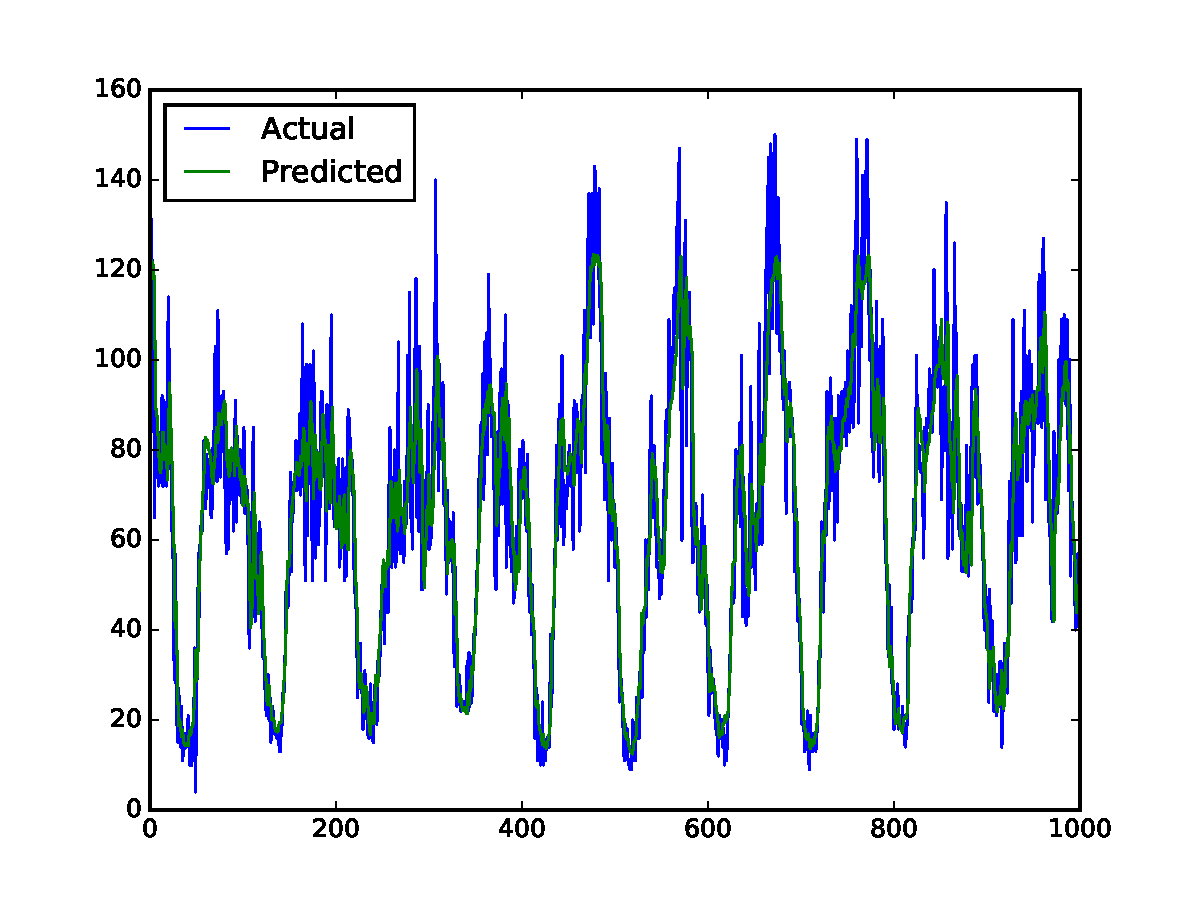
\includegraphics[width=\textwidth,height=\textheight,keepaspectratio]{Figures/lstm.pdf}
    \rule{35em}{0.5pt}
  \caption[LSTM - Actual vs Predictions]{Long Short Term Memory predictions vs actual test data for
  1000 observations.}
  \label{fig:LstmActualPredicted}
\end{figure}
\section{Evaluation}

Comparision of the LSTM model with the following models

\begin{itemize}
\item Exponential smoothing
\item ARIMA
\item K-Nearest Neighbour
\item Backpropagation Neural Network
\item Radial Basis Function(RBF) NN model
\item Stacked Autoencoders
\end{itemize}

The accuracy scores are - MAE, MRE and RMSE